\documentclass{whiteboard}
\begin{document}
\begin{frame}[plain,t]
\bbcover{Codeforces Round \#250 (Div. 2)}{Problem C -- The Child and Toy}{Prof. Edson Alves}{Faculdade UnB Gama}

\end{frame}
\begin{frame}[plain,t]
\vspace*{\fill}

\bbenglish{On Children's Day, the child got a toy from Delayyy as a present. However, the child is so naughty that he can't wait to destroy the toy.}

\vspace{0.1in}

\bbenglish{The toy consists of $n$ parts and $m$ ropes. Each rope links two parts, but every pair of parts is linked by at most one rope. To split the toy, the child must remove all its parts. The child can remove a single part at a time, and each remove consume an energy. Let's define an energy value of part $i$ as $v_i$. The child spend $v_{f_1} + v_{f_2} + \ldots + v_{f_k}$ energy for removing part $i$ where $f_1, f_2, \ldots, f_k$ are the parts that are directly connected to the $i$-th and haven't been removed.}

\vspace{0.1in}

\bbenglish{Help the child to find out, what is the minimum total energy he should spend to remove all $n$ parts.}

\vspace*{\fill}
\end{frame}
\begin{frame}[plain,t]
\vspace*{\fill}

\bbtext{No Dia das Crianças, a criança ganha um brinquedo from Delayyy como presente. Contudo, a criança é tão levada que ela não pode esperar para destruir o brinquedo.}

\vspace{0.1in}

\bbtext{O brinquedo é formado por $n$ partes e $m$ cordas. Cada corda une duas partes, mas cada par de partes é unido por, no máximo, uma corda. Para quebrar o brinquedo, a criança deve remover todas as suas partes. A criança pode remover uma única parte por vez, e cada remoção consome energia. Vamos define a energia da parte $i$ como $v_i$. A criança gasta energia igual a $v_{f_1} + v_{f_2} + \ldots + v_{f_k}$ para remover a parte $i$, onde  $f_1, f_2, \ldots, f_k$ são as partes que estão diretamente conectadas à $i$-ésima parte e que não foram removidas ainda.}

\vspace{0.1in}

\bbtext{Auxilie a criança a descobir qual é o total mínimo de energia que ela deve gastar para remover todas as $n$ partes.}

\vspace*{\fill}
\end{frame}
\begin{frame}[plain,t]
\vspace*{\fill}

\bbbold{Input}

\vspace{0.1in}

\bbenglish{The first line contains two integers $n$ and $m$ $(1\leq n\leq 1000; 0\leq m\leq 2000)$. The second line contains $n$ integers: $v_1, v_2, \ldots, v_n$ $(0\leq v_i\leq 10^5)$. Then followed $m$ lines, each line contains two integers $x_i$ and $y_i$, representing a rope from part $x_i$ to part $y_i$ $(1\leq x_i, y_i\leq n; x_i\neq y_i)$.}

\vspace{0.1in}

\bbenglish{Consider all the parts are numbered from $1$ to $n$.}

\vspace{0.2in}

\bbbold{Output}

\vspace{0.1in}

\bbenglish{Output the minimum total energy the child should spend to remove all $n$ parts of the toy.}

\vspace*{\fill}
\end{frame}
\begin{frame}[plain,t]
\vspace*{\fill}

\bbbold{Entrada}

\vspace{0.1in}

\bbtext{A primeira linha contém dois inteiros $n$ e $m$ $(1\leq n\leq 1000; 0\leq m\leq 2000)$. A segunda linha contém $n$ inteiros: $v_1, v_2, \ldots, v_n$ $(0\leq v_i\leq 10^5)$. Então seguem $m$ linhas, e cada linha contém dois inteiros $x_i$ e $y_i$, representando uma corda da parte $x_i$ para a parte $y_i$ $(1\leq x_i, y_i\leq n; x_i\neq y_i)$.}

\vspace{0.1in}

\bbtext{Considere que todas as partes são numeradas de $1$ a $n$.}

\vspace{0.2in}

\bbbold{Saída}

\vspace{0.1in}

\bbtext{Imprima o total mínimo de energia que a criança deveria gastar para remover todas as $n$ partes do brinquedo.}

\vspace*{\fill}
\end{frame}
\begin{frame}[plain,t]
\begin{tikzpicture}
\node[draw,opacity=0] at (0, 0) {x};
\node[draw,opacity=0] at (14, 8) {x};

	\node[anchor=west] (header) at (0, 7.0) { \bbbold{Exemplo de entrada e saída} };

\end{tikzpicture}
\end{frame}
\begin{frame}[plain,t]
\begin{tikzpicture}
\node[draw,opacity=0] at (0, 0) {x};
\node[draw,opacity=0] at (14, 8) {x};

	\node[anchor=west] (header) at (0, 7.0) { \bbbold{Exemplo de entrada e saída} };


	\node[anchor=west] (line1) at (1.0, 6.0) { \bbtext{\texttt{4 3} } };

\end{tikzpicture}
\end{frame}
\begin{frame}[plain,t]
\begin{tikzpicture}
\node[draw,opacity=0] at (0, 0) {x};
\node[draw,opacity=0] at (14, 8) {x};

	\node[anchor=west] (header) at (0, 7.0) { \bbbold{Exemplo de entrada e saída} };


	\node[anchor=west] (line1) at (1.0, 6.0) { \bbtext{\texttt{4 3} } };


	\draw[->,color=BBViolet] (1.25, 5.0) to  (1.25, 5.75);

	\node[] (r) at (1.25, 4.75) { \footnotesize \bbcomment{\# número de partes} };

\end{tikzpicture}
\end{frame}
\begin{frame}[plain,t]
\begin{tikzpicture}
\node[draw,opacity=0] at (0, 0) {x};
\node[draw,opacity=0] at (14, 8) {x};

	\node[anchor=west] (header) at (0, 7.0) { \bbbold{Exemplo de entrada e saída} };


	\node[anchor=west] (line1) at (1.0, 6.0) { \bbtext{\texttt{4 3} } };


	\draw[->,color=BBViolet] (1.65, 5.0) to  (1.65, 5.75);

	\node[] (r) at (1.65, 4.75) { \footnotesize \bbcomment{\# número de cordas} };



\end{tikzpicture}
\end{frame}
\begin{frame}[plain,t]
\begin{tikzpicture}
\node[draw,opacity=0] at (0, 0) {x};
\node[draw,opacity=0] at (14, 8) {x};

	\node[anchor=west] (header) at (0, 7.0) { \bbbold{Exemplo de entrada e saída} };


	\node[anchor=west] (line1) at (1.0, 6.0) { \bbtext{\texttt{4 3} } };







	\node[draw,very thick,circle] (node1) at (7.0, 4.0) { \bbtext{1} };

	\node[draw,very thick,circle] (node2) at (10.0, 7.0) { \bbtext{2} };

	\node[draw,very thick,circle] (node3) at (13.0, 4.0) { \bbtext{3} };

	\node[draw,very thick,circle] (node4) at (10.0, 1.0) { \bbtext{4} };

\end{tikzpicture}
\end{frame}
\begin{frame}[plain,t]
\begin{tikzpicture}
\node[draw,opacity=0] at (0, 0) {x};
\node[draw,opacity=0] at (14, 8) {x};

	\node[anchor=west] (header) at (0, 7.0) { \bbbold{Exemplo de entrada e saída} };


	\node[anchor=west] (line1) at (1.0, 6.0) { \bbtext{\texttt{4 3} } };







	\node[draw,very thick,circle] (node1) at (7.0, 4.0) { \bbtext{1} };

	\node[draw,very thick,circle] (node2) at (10.0, 7.0) { \bbtext{2} };

	\node[draw,very thick,circle] (node3) at (13.0, 4.0) { \bbtext{3} };

	\node[draw,very thick,circle] (node4) at (10.0, 1.0) { \bbtext{4} };


	\node[anchor=west] (line2) at (1.0, 5.5) { \bbtext{\texttt{10 20 30 40} } };

\end{tikzpicture}
\end{frame}
\begin{frame}[plain,t]
\begin{tikzpicture}
\node[draw,opacity=0] at (0, 0) {x};
\node[draw,opacity=0] at (14, 8) {x};

	\node[anchor=west] (header) at (0, 7.0) { \bbbold{Exemplo de entrada e saída} };


	\node[anchor=west] (line1) at (1.0, 6.0) { \bbtext{\texttt{4 3} } };


	\draw[->,color=BBViolet] (1.35, 5.25) to  (1.35, 4.25);

	\node[] (r) at (1.35, 4.0) { \footnotesize $v_1$ };




	\node[draw,very thick,circle] (node1) at (7.0, 4.0) { \bbtext{1} };

	\node[draw,very thick,circle] (node2) at (10.0, 7.0) { \bbtext{2} };

	\node[draw,very thick,circle] (node3) at (13.0, 4.0) { \bbtext{3} };

	\node[draw,very thick,circle] (node4) at (10.0, 1.0) { \bbtext{4} };


	\node[anchor=west] (line2) at (1.0, 5.5) { \bbtext{\texttt{10 20 30 40} } };




\end{tikzpicture}
\end{frame}
\begin{frame}[plain,t]
\begin{tikzpicture}
\node[draw,opacity=0] at (0, 0) {x};
\node[draw,opacity=0] at (14, 8) {x};

	\node[anchor=west] (header) at (0, 7.0) { \bbbold{Exemplo de entrada e saída} };


	\node[anchor=west] (line1) at (1.0, 6.0) { \bbtext{\texttt{4 3} } };


	\draw[->,color=BBViolet] (1.95, 5.25) to  (1.95, 4.25);

	\node[] (r) at (1.95, 4.0) { \footnotesize $v_2$ };




	\node[draw,very thick,circle] (node1) at (7.0, 4.0) { \bbtext{1} };

	\node[draw,very thick,circle] (node2) at (10.0, 7.0) { \bbtext{2} };

	\node[draw,very thick,circle] (node3) at (13.0, 4.0) { \bbtext{3} };

	\node[draw,very thick,circle] (node4) at (10.0, 1.0) { \bbtext{4} };


	\node[anchor=west] (line2) at (1.0, 5.5) { \bbtext{\texttt{10 20 30 40} } };







\end{tikzpicture}
\end{frame}
\begin{frame}[plain,t]
\begin{tikzpicture}
\node[draw,opacity=0] at (0, 0) {x};
\node[draw,opacity=0] at (14, 8) {x};

	\node[anchor=west] (header) at (0, 7.0) { \bbbold{Exemplo de entrada e saída} };


	\node[anchor=west] (line1) at (1.0, 6.0) { \bbtext{\texttt{4 3} } };


	\draw[->,color=BBViolet] (2.55, 5.25) to  (2.55, 4.25);

	\node[] (r) at (2.55, 4.0) { \footnotesize $v_3$ };




	\node[draw,very thick,circle] (node1) at (7.0, 4.0) { \bbtext{1} };

	\node[draw,very thick,circle] (node2) at (10.0, 7.0) { \bbtext{2} };

	\node[draw,very thick,circle] (node3) at (13.0, 4.0) { \bbtext{3} };

	\node[draw,very thick,circle] (node4) at (10.0, 1.0) { \bbtext{4} };


	\node[anchor=west] (line2) at (1.0, 5.5) { \bbtext{\texttt{10 20 30 40} } };









\end{tikzpicture}
\end{frame}
\begin{frame}[plain,t]
\begin{tikzpicture}
\node[draw,opacity=0] at (0, 0) {x};
\node[draw,opacity=0] at (14, 8) {x};

	\node[anchor=west] (header) at (0, 7.0) { \bbbold{Exemplo de entrada e saída} };


	\node[anchor=west] (line1) at (1.0, 6.0) { \bbtext{\texttt{4 3} } };


	\draw[->,color=BBViolet] (3.15, 5.25) to  (3.15, 4.25);

	\node[] (r) at (3.15, 4.0) { \footnotesize $v_4$ };




	\node[draw,very thick,circle] (node1) at (7.0, 4.0) { \bbtext{1} };

	\node[draw,very thick,circle] (node2) at (10.0, 7.0) { \bbtext{2} };

	\node[draw,very thick,circle] (node3) at (13.0, 4.0) { \bbtext{3} };

	\node[draw,very thick,circle] (node4) at (10.0, 1.0) { \bbtext{4} };


	\node[anchor=west] (line2) at (1.0, 5.5) { \bbtext{\texttt{10 20 30 40} } };











\end{tikzpicture}
\end{frame}
\begin{frame}[plain,t]
\begin{tikzpicture}
\node[draw,opacity=0] at (0, 0) {x};
\node[draw,opacity=0] at (14, 8) {x};

	\node[anchor=west] (header) at (0, 7.0) { \bbbold{Exemplo de entrada e saída} };


	\node[anchor=west] (line1) at (1.0, 6.0) { \bbtext{\texttt{4 3} } };







	\node[draw,very thick,circle] (node1) at (7.0, 4.0) { \bbtext{1}$_{10}$ };

	\node[draw,very thick,circle] (node2) at (10.0, 7.0) { \bbtext{2}$_{20}$ };

	\node[draw,very thick,circle] (node3) at (13.0, 4.0) { \bbtext{3}$_{30}$ };

	\node[draw,very thick,circle] (node4) at (10.0, 1.0) { \bbtext{4}$_{40}$ };


	\node[anchor=west] (line2) at (1.0, 5.5) { \bbtext{\texttt{10 20 30 40} } };













\end{tikzpicture}
\end{frame}
\begin{frame}[plain,t]
\begin{tikzpicture}
\node[draw,opacity=0] at (0, 0) {x};
\node[draw,opacity=0] at (14, 8) {x};

	\node[anchor=west] (header) at (0, 7.0) { \bbbold{Exemplo de entrada e saída} };


	\node[anchor=west] (line1) at (1.0, 6.0) { \bbtext{\texttt{4 3} } };







	\node[draw,very thick,circle] (node1) at (7.0, 4.0) { \bbtext{1}$_{10}$ };

	\node[draw,very thick,circle] (node2) at (10.0, 7.0) { \bbtext{2}$_{20}$ };

	\node[draw,very thick,circle] (node3) at (13.0, 4.0) { \bbtext{3}$_{30}$ };

	\node[draw,very thick,circle] (node4) at (10.0, 1.0) { \bbtext{4}$_{40}$ };


	\node[anchor=west] (line2) at (1.0, 5.5) { \bbtext{\texttt{10 20 30 40} } };














	\node[anchor=west] (line3) at (1.0, 5.0) { \bbtext{\texttt{1 4} } };


\end{tikzpicture}
\end{frame}
\begin{frame}[plain,t]
\begin{tikzpicture}
\node[draw,opacity=0] at (0, 0) {x};
\node[draw,opacity=0] at (14, 8) {x};

	\node[anchor=west] (header) at (0, 7.0) { \bbbold{Exemplo de entrada e saída} };


	\node[anchor=west] (line1) at (1.0, 6.0) { \bbtext{\texttt{4 3} } };


	\draw[->,color=BBViolet] (1.45, 4.75) to  (1.45, 3.75);

	\node[] (r) at (1.45, 3.5) { \footnotesize \bbcomment{corda} };




	\node[draw,very thick,circle] (node1) at (7.0, 4.0) { \bbtext{1}$_{10}$ };

	\node[draw,very thick,circle] (node2) at (10.0, 7.0) { \bbtext{2}$_{20}$ };

	\node[draw,very thick,circle] (node3) at (13.0, 4.0) { \bbtext{3}$_{30}$ };

	\node[draw,very thick,circle] (node4) at (10.0, 1.0) { \bbtext{4}$_{40}$ };


	\node[anchor=west] (line2) at (1.0, 5.5) { \bbtext{\texttt{10 20 30 40} } };














	\node[anchor=west] (line3) at (1.0, 5.0) { \bbtext{\texttt{1 4} } };





\end{tikzpicture}
\end{frame}
\begin{frame}[plain,t]
\begin{tikzpicture}
\node[draw,opacity=0] at (0, 0) {x};
\node[draw,opacity=0] at (14, 8) {x};

	\node[anchor=west] (header) at (0, 7.0) { \bbbold{Exemplo de entrada e saída} };


	\node[anchor=west] (line1) at (1.0, 6.0) { \bbtext{\texttt{4 3} } };







	\node[draw,very thick,circle] (node1) at (7.0, 4.0) { \bbtext{1}$_{10}$ };

	\node[draw,very thick,circle] (node2) at (10.0, 7.0) { \bbtext{2}$_{20}$ };

	\node[draw,very thick,circle] (node3) at (13.0, 4.0) { \bbtext{3}$_{30}$ };

	\node[draw,very thick,circle] (node4) at (10.0, 1.0) { \bbtext{4}$_{40}$ };


	\node[anchor=west] (line2) at (1.0, 5.5) { \bbtext{\texttt{10 20 30 40} } };














	\node[anchor=west] (line3) at (1.0, 5.0) { \bbtext{\texttt{1 4} } };






	\draw[thick](node1) to (node4);

\end{tikzpicture}
\end{frame}
\begin{frame}[plain,t]
\begin{tikzpicture}
\node[draw,opacity=0] at (0, 0) {x};
\node[draw,opacity=0] at (14, 8) {x};

	\node[anchor=west] (header) at (0, 7.0) { \bbbold{Exemplo de entrada e saída} };


	\node[anchor=west] (line1) at (1.0, 6.0) { \bbtext{\texttt{4 3} } };







	\node[draw,very thick,circle] (node1) at (7.0, 4.0) { \bbtext{1}$_{10}$ };

	\node[draw,very thick,circle] (node2) at (10.0, 7.0) { \bbtext{2}$_{20}$ };

	\node[draw,very thick,circle] (node3) at (13.0, 4.0) { \bbtext{3}$_{30}$ };

	\node[draw,very thick,circle] (node4) at (10.0, 1.0) { \bbtext{4}$_{40}$ };


	\node[anchor=west] (line2) at (1.0, 5.5) { \bbtext{\texttt{10 20 30 40} } };














	\node[anchor=west] (line3) at (1.0, 5.0) { \bbtext{\texttt{1 4} } };






	\draw[thick](node1) to (node4);


	\node[anchor=west] (line4) at (1.0, 4.5) { \bbtext{\texttt{1 2} } };

\end{tikzpicture}
\end{frame}
\begin{frame}[plain,t]
\begin{tikzpicture}
\node[draw,opacity=0] at (0, 0) {x};
\node[draw,opacity=0] at (14, 8) {x};

	\node[anchor=west] (header) at (0, 7.0) { \bbbold{Exemplo de entrada e saída} };


	\node[anchor=west] (line1) at (1.0, 6.0) { \bbtext{\texttt{4 3} } };







	\node[draw,very thick,circle] (node1) at (7.0, 4.0) { \bbtext{1}$_{10}$ };

	\node[draw,very thick,circle] (node2) at (10.0, 7.0) { \bbtext{2}$_{20}$ };

	\node[draw,very thick,circle] (node3) at (13.0, 4.0) { \bbtext{3}$_{30}$ };

	\node[draw,very thick,circle] (node4) at (10.0, 1.0) { \bbtext{4}$_{40}$ };


	\node[anchor=west] (line2) at (1.0, 5.5) { \bbtext{\texttt{10 20 30 40} } };














	\node[anchor=west] (line3) at (1.0, 5.0) { \bbtext{\texttt{1 4} } };






	\draw[thick](node1) to (node4);


	\node[anchor=west] (line4) at (1.0, 4.5) { \bbtext{\texttt{1 2} } };


	\draw[thick](node1) to (node2);

\end{tikzpicture}
\end{frame}
\begin{frame}[plain,t]
\begin{tikzpicture}
\node[draw,opacity=0] at (0, 0) {x};
\node[draw,opacity=0] at (14, 8) {x};

	\node[anchor=west] (header) at (0, 7.0) { \bbbold{Exemplo de entrada e saída} };


	\node[anchor=west] (line1) at (1.0, 6.0) { \bbtext{\texttt{4 3} } };







	\node[draw,very thick,circle] (node1) at (7.0, 4.0) { \bbtext{1}$_{10}$ };

	\node[draw,very thick,circle] (node2) at (10.0, 7.0) { \bbtext{2}$_{20}$ };

	\node[draw,very thick,circle] (node3) at (13.0, 4.0) { \bbtext{3}$_{30}$ };

	\node[draw,very thick,circle] (node4) at (10.0, 1.0) { \bbtext{4}$_{40}$ };


	\node[anchor=west] (line2) at (1.0, 5.5) { \bbtext{\texttt{10 20 30 40} } };














	\node[anchor=west] (line3) at (1.0, 5.0) { \bbtext{\texttt{1 4} } };






	\draw[thick](node1) to (node4);


	\node[anchor=west] (line4) at (1.0, 4.5) { \bbtext{\texttt{1 2} } };


	\draw[thick](node1) to (node2);


	\node[anchor=west] (line5) at (1.0, 4.0) { \bbtext{\texttt{2 3} } };

\end{tikzpicture}
\end{frame}
\begin{frame}[plain,t]
\begin{tikzpicture}
\node[draw,opacity=0] at (0, 0) {x};
\node[draw,opacity=0] at (14, 8) {x};

	\node[anchor=west] (header) at (0, 7.0) { \bbbold{Exemplo de entrada e saída} };


	\node[anchor=west] (line1) at (1.0, 6.0) { \bbtext{\texttt{4 3} } };







	\node[draw,very thick,circle] (node1) at (7.0, 4.0) { \bbtext{1}$_{10}$ };

	\node[draw,very thick,circle] (node2) at (10.0, 7.0) { \bbtext{2}$_{20}$ };

	\node[draw,very thick,circle] (node3) at (13.0, 4.0) { \bbtext{3}$_{30}$ };

	\node[draw,very thick,circle] (node4) at (10.0, 1.0) { \bbtext{4}$_{40}$ };


	\node[anchor=west] (line2) at (1.0, 5.5) { \bbtext{\texttt{10 20 30 40} } };














	\node[anchor=west] (line3) at (1.0, 5.0) { \bbtext{\texttt{1 4} } };






	\draw[thick](node1) to (node4);


	\node[anchor=west] (line4) at (1.0, 4.5) { \bbtext{\texttt{1 2} } };


	\draw[thick](node1) to (node2);


	\node[anchor=west] (line5) at (1.0, 4.0) { \bbtext{\texttt{2 3} } };


	\draw[thick](node2) to (node3);

\end{tikzpicture}
\end{frame}
\begin{frame}[plain,t]
\begin{tikzpicture}
\node[draw,opacity=0] at (0, 0) {x};
\node[draw,opacity=0] at (14, 8) {x};

	\node[anchor=west] (header) at (0, 7.0) { \bbbold{Exemplo de entrada e saída} };


	\node[anchor=west] (line1) at (1.0, 6.0) { \bbtext{\texttt{4 3} } };







	\node[draw,very thick,circle] (node1) at (7.0, 4.0) { \bbtext{1}$_{10}$ };

	\node[draw,very thick,circle] (node2) at (10.0, 7.0) { \bbtext{2}$_{20}$ };

	\node[draw,very thick,circle] (node3) at (13.0, 4.0) { \bbtext{3}$_{30}$ };

	\node[draw,very thick,circle] (node4) at (10.0, 1.0) { \bbtext{4}$_{40}$ };


	\node[anchor=west] (line2) at (1.0, 5.5) { \bbtext{\texttt{10 20 30 40} } };














	\node[anchor=west] (line3) at (1.0, 5.0) { \bbtext{\texttt{1 4} } };






	\draw[thick](node1) to node { \Large \textbf{\textcolor{BBRed}{x}} } node[above right] { \bbinfo { 10 } } (node4);


	\node[anchor=west] (line4) at (1.0, 4.5) { \bbtext{\texttt{1 2} } };


	\draw[thick](node1) to (node2);


	\node[anchor=west] (line5) at (1.0, 4.0) { \bbtext{\texttt{2 3} } };


	\draw[thick](node2) to (node3);



\end{tikzpicture}
\end{frame}
\begin{frame}[plain,t]
\begin{tikzpicture}
\node[draw,opacity=0] at (0, 0) {x};
\node[draw,opacity=0] at (14, 8) {x};

	\node[anchor=west] (header) at (0, 7.0) { \bbbold{Exemplo de entrada e saída} };


	\node[anchor=west] (line1) at (1.0, 6.0) { \bbtext{\texttt{4 3} } };







	\node[draw,very thick,circle] (node1) at (7.0, 4.0) { \bbtext{1}$_{10}$ };

	\node[draw,very thick,circle] (node2) at (10.0, 7.0) { \bbtext{2}$_{20}$ };

	\node[draw,very thick,circle] (node3) at (13.0, 4.0) { \bbtext{3}$_{30}$ };



	\node[anchor=west] (line2) at (1.0, 5.5) { \bbtext{\texttt{10 20 30 40} } };














	\node[anchor=west] (line3) at (1.0, 5.0) { \bbtext{\texttt{1 4} } };








	\node[anchor=west] (line4) at (1.0, 4.5) { \bbtext{\texttt{1 2} } };


	\draw[thick](node1) to (node2);


	\node[anchor=west] (line5) at (1.0, 4.0) { \bbtext{\texttt{2 3} } };


	\draw[thick](node2) to (node3);




\end{tikzpicture}
\end{frame}
\begin{frame}[plain,t]
\begin{tikzpicture}
\node[draw,opacity=0] at (0, 0) {x};
\node[draw,opacity=0] at (14, 8) {x};

	\node[anchor=west] (header) at (0, 7.0) { \bbbold{Exemplo de entrada e saída} };


	\node[anchor=west] (line1) at (1.0, 6.0) { \bbtext{\texttt{4 3} } };







	\node[draw,very thick,circle] (node1) at (7.0, 4.0) { \bbtext{1}$_{10}$ };

	\node[draw,very thick,circle] (node2) at (10.0, 7.0) { \bbtext{2}$_{20}$ };

	\node[draw,very thick,circle] (node3) at (13.0, 4.0) { \bbtext{3}$_{30}$ };



	\node[anchor=west] (line2) at (1.0, 5.5) { \bbtext{\texttt{10 20 30 40} } };














	\node[anchor=west] (line3) at (1.0, 5.0) { \bbtext{\texttt{1 4} } };








	\node[anchor=west] (line4) at (1.0, 4.5) { \bbtext{\texttt{1 2} } };


	\draw[thick](node1) to (node2);


	\node[anchor=west] (line5) at (1.0, 4.0) { \bbtext{\texttt{2 3} } };


	\draw[thick](node2) to node { \Large \textbf{\textcolor{BBRed}{x}} } node[above right] { \bbinfo { 20 } } (node3);





\end{tikzpicture}
\end{frame}
\begin{frame}[plain,t]
\begin{tikzpicture}
\node[draw,opacity=0] at (0, 0) {x};
\node[draw,opacity=0] at (14, 8) {x};

	\node[anchor=west] (header) at (0, 7.0) { \bbbold{Exemplo de entrada e saída} };


	\node[anchor=west] (line1) at (1.0, 6.0) { \bbtext{\texttt{4 3} } };







	\node[draw,very thick,circle] (node1) at (7.0, 4.0) { \bbtext{1}$_{10}$ };

	\node[draw,very thick,circle] (node2) at (10.0, 7.0) { \bbtext{2}$_{20}$ };




	\node[anchor=west] (line2) at (1.0, 5.5) { \bbtext{\texttt{10 20 30 40} } };














	\node[anchor=west] (line3) at (1.0, 5.0) { \bbtext{\texttt{1 4} } };








	\node[anchor=west] (line4) at (1.0, 4.5) { \bbtext{\texttt{1 2} } };


	\draw[thick](node1) to (node2);


	\node[anchor=west] (line5) at (1.0, 4.0) { \bbtext{\texttt{2 3} } };









\end{tikzpicture}
\end{frame}
\begin{frame}[plain,t]
\begin{tikzpicture}
\node[draw,opacity=0] at (0, 0) {x};
\node[draw,opacity=0] at (14, 8) {x};

	\node[anchor=west] (header) at (0, 7.0) { \bbbold{Exemplo de entrada e saída} };


	\node[anchor=west] (line1) at (1.0, 6.0) { \bbtext{\texttt{4 3} } };







	\node[draw,very thick,circle] (node1) at (7.0, 4.0) { \bbtext{1}$_{10}$ };

	\node[draw,very thick,circle] (node2) at (10.0, 7.0) { \bbtext{2}$_{20}$ };




	\node[anchor=west] (line2) at (1.0, 5.5) { \bbtext{\texttt{10 20 30 40} } };














	\node[anchor=west] (line3) at (1.0, 5.0) { \bbtext{\texttt{1 4} } };








	\node[anchor=west] (line4) at (1.0, 4.5) { \bbtext{\texttt{1 2} } };


	\draw[thick](node1) to node { \Large \textbf{\textcolor{BBRed}{x}} } node[above left] { \bbinfo { 10 } } (node2);


	\node[anchor=west] (line5) at (1.0, 4.0) { \bbtext{\texttt{2 3} } };










\end{tikzpicture}
\end{frame}
\begin{frame}[plain,t]
\begin{tikzpicture}
\node[draw,opacity=0] at (0, 0) {x};
\node[draw,opacity=0] at (14, 8) {x};

	\node[anchor=west] (header) at (0, 7.0) { \bbbold{Exemplo de entrada e saída} };


	\node[anchor=west] (line1) at (1.0, 6.0) { \bbtext{\texttt{4 3} } };







	\node[draw,very thick,circle] (node1) at (7.0, 4.0) { \bbtext{1}$_{10}$ };





	\node[anchor=west] (line2) at (1.0, 5.5) { \bbtext{\texttt{10 20 30 40} } };














	\node[anchor=west] (line3) at (1.0, 5.0) { \bbtext{\texttt{1 4} } };








	\node[anchor=west] (line4) at (1.0, 4.5) { \bbtext{\texttt{1 2} } };




	\node[anchor=west] (line5) at (1.0, 4.0) { \bbtext{\texttt{2 3} } };











\end{tikzpicture}
\end{frame}
\begin{frame}[plain,t]
\begin{tikzpicture}
\node[draw,opacity=0] at (0, 0) {x};
\node[draw,opacity=0] at (14, 8) {x};

	\node[anchor=west] (header) at (0, 7.0) { \bbbold{Exemplo de entrada e saída} };


	\node[anchor=west] (line1) at (1.0, 6.0) { \bbtext{\texttt{4 3} } };












	\node[anchor=west] (line2) at (1.0, 5.5) { \bbtext{\texttt{10 20 30 40} } };














	\node[anchor=west] (line3) at (1.0, 5.0) { \bbtext{\texttt{1 4} } };








	\node[anchor=west] (line4) at (1.0, 4.5) { \bbtext{\texttt{1 2} } };




	\node[anchor=west] (line5) at (1.0, 4.0) { \bbtext{\texttt{2 3} } };












\end{tikzpicture}
\end{frame}
\begin{frame}[plain,t]
\begin{tikzpicture}
\node[draw,opacity=0] at (0, 0) {x};
\node[draw,opacity=0] at (14, 8) {x};

	\node[anchor=west] (header) at (0, 7.0) { \bbbold{Exemplo de entrada e saída} };


	\node[anchor=west] (line1) at (1.0, 6.0) { \bbtext{\texttt{4 3} } };


	\draw[->,color=BBBlack,-latex,very thick] (1.45, 3.75) to  (1.45, 2.75);

	\node[] (r) at (1.45, 2.5) { \bbinfo{40} };









	\node[anchor=west] (line2) at (1.0, 5.5) { \bbtext{\texttt{10 20 30 40} } };














	\node[anchor=west] (line3) at (1.0, 5.0) { \bbtext{\texttt{1 4} } };








	\node[anchor=west] (line4) at (1.0, 4.5) { \bbtext{\texttt{1 2} } };




	\node[anchor=west] (line5) at (1.0, 4.0) { \bbtext{\texttt{2 3} } };















\end{tikzpicture}
\end{frame}
\begin{frame}[plain,t]
\begin{tikzpicture}
\node[draw,opacity=0] at (0, 0) {x};
\node[draw,opacity=0] at (14, 8) {x};

	\node[anchor=west] (header) at (0, 7.0) { \bbbold{Exemplo de entrada e saída} };

\end{tikzpicture}
\end{frame}
\begin{frame}[plain,t]
\begin{tikzpicture}
\node[draw,opacity=0] at (0, 0) {x};
\node[draw,opacity=0] at (14, 8) {x};

	\node[anchor=west] (header) at (0, 7.0) { \bbbold{Exemplo de entrada e saída} };


	\node[anchor=west] (line1) at (1.0, 6.0) { \bbtext{\texttt{7 10} } };

\end{tikzpicture}
\end{frame}
\begin{frame}[plain,t]
\begin{tikzpicture}
\node[draw,opacity=0] at (0, 0) {x};
\node[draw,opacity=0] at (14, 8) {x};

	\node[anchor=west] (header) at (0, 7.0) { \bbbold{Exemplo de entrada e saída} };


	\node[anchor=west] (line1) at (1.0, 6.0) { \bbtext{\texttt{7 10} } };


	\node[draw,very thick,circle] (node1) at (6.0, 5.0) { \bbtext{1} };

	\node[draw,very thick,circle] (node2) at (8.0, 7.0) { \bbtext{2} };

	\node[draw,very thick,circle] (node3) at (10.0, 7.0) { \bbtext{3} };

	\node[draw,very thick,circle] (node4) at (12.0, 4.0) { \bbtext{4} };

	\node[draw,very thick,circle] (node5) at (10.0, 1.0) { \bbtext{5} };

	\node[draw,very thick,circle] (node6) at (8.0, 1.0) { \bbtext{6} };

	\node[draw,very thick,circle] (node7) at (6.0, 3.0) { \bbtext{7} };

\end{tikzpicture}
\end{frame}
\begin{frame}[plain,t]
\begin{tikzpicture}
\node[draw,opacity=0] at (0, 0) {x};
\node[draw,opacity=0] at (14, 8) {x};

	\node[anchor=west] (header) at (0, 7.0) { \bbbold{Exemplo de entrada e saída} };


	\node[anchor=west] (line1) at (1.0, 6.0) { \bbtext{\texttt{7 10} } };


	\node[draw,very thick,circle] (node1) at (6.0, 5.0) { \bbtext{1} };

	\node[draw,very thick,circle] (node2) at (8.0, 7.0) { \bbtext{2} };

	\node[draw,very thick,circle] (node3) at (10.0, 7.0) { \bbtext{3} };

	\node[draw,very thick,circle] (node4) at (12.0, 4.0) { \bbtext{4} };

	\node[draw,very thick,circle] (node5) at (10.0, 1.0) { \bbtext{5} };

	\node[draw,very thick,circle] (node6) at (8.0, 1.0) { \bbtext{6} };

	\node[draw,very thick,circle] (node7) at (6.0, 3.0) { \bbtext{7} };


	\node[anchor=west] (line2) at (1.0, 5.5) { \bbtext{\texttt{40 10 20 10 20 80 40}} };

\end{tikzpicture}
\end{frame}
\begin{frame}[plain,t]
\begin{tikzpicture}
\node[draw,opacity=0] at (0, 0) {x};
\node[draw,opacity=0] at (14, 8) {x};

	\node[anchor=west] (header) at (0, 7.0) { \bbbold{Exemplo de entrada e saída} };


	\node[anchor=west] (line1) at (1.0, 6.0) { \bbtext{\texttt{7 10} } };


	\node[draw,very thick,circle] (node1) at (6.0, 5.0) { \footnosize \bbtext{1}$_40$ };

	\node[draw,very thick,circle] (node2) at (8.0, 7.0) { \bbtext{2} };

	\node[draw,very thick,circle] (node3) at (10.0, 7.0) { \bbtext{3} };

	\node[draw,very thick,circle] (node4) at (12.0, 4.0) { \bbtext{4} };

	\node[draw,very thick,circle] (node5) at (10.0, 1.0) { \bbtext{5} };

	\node[draw,very thick,circle] (node6) at (8.0, 1.0) { \bbtext{6} };

	\node[draw,very thick,circle] (node7) at (6.0, 3.0) { \bbtext{7} };


	\node[anchor=west] (line2) at (1.0, 5.5) { \bbtext{\texttt{40 10 20 10 20 80 40}} };


\end{tikzpicture}
\end{frame}
\begin{frame}[plain,t]
\begin{tikzpicture}
\node[draw,opacity=0] at (0, 0) {x};
\node[draw,opacity=0] at (14, 8) {x};

	\node[anchor=west] (header) at (0, 6.0) { \Large \bbbold{Solução} };

\end{tikzpicture}
\end{frame}
\begin{frame}[plain,t]
\begin{tikzpicture}
\node[draw,opacity=0] at (0, 0) {x};
\node[draw,opacity=0] at (14, 8) {x};

	\node[anchor=west] (header) at (0, 6.0) { \Large \bbbold{Solução} };


	\node[anchor=west] (a) at (1.0, 5.0) { $\star$ \bbtext{Cada viagem consiste em um problema de caminho mínimo} };

\end{tikzpicture}
\end{frame}
\begin{frame}[plain,t]
\begin{tikzpicture}
\node[draw,opacity=0] at (0, 0) {x};
\node[draw,opacity=0] at (14, 8) {x};

	\node[anchor=west] (header) at (0, 6.0) { \Large \bbbold{Solução} };


	\node[anchor=west] (a) at (1.0, 5.0) { $\star$ \bbtext{Cada viagem consiste em um problema de caminho mínimo} };


	\node[anchor=west] (b) at (1.0, 4.0) { $\star$ \bbtext{As arestas tem peso $1$, exceto a direção da corrente, que tem peso $0$} };

\end{tikzpicture}
\end{frame}
\begin{frame}[plain,t]
\begin{tikzpicture}
\node[draw,opacity=0] at (0, 0) {x};
\node[draw,opacity=0] at (14, 8) {x};

	\node[anchor=west] (header) at (0, 6.0) { \Large \bbbold{Solução} };


	\node[anchor=west] (a) at (1.0, 5.0) { $\star$ \bbtext{Cada viagem consiste em um problema de caminho mínimo} };


	\node[anchor=west] (b) at (1.0, 4.0) { $\star$ \bbtext{As arestas tem peso $1$, exceto a direção da corrente, que tem peso $0$} };


	\node[anchor=west] (c) at (1.0, 3.0) { $\star$ \bbtext{Portanto o problema pode ser resolvido por meio de uma BFS 0/1} };

\end{tikzpicture}
\end{frame}
\begin{frame}[plain,t]
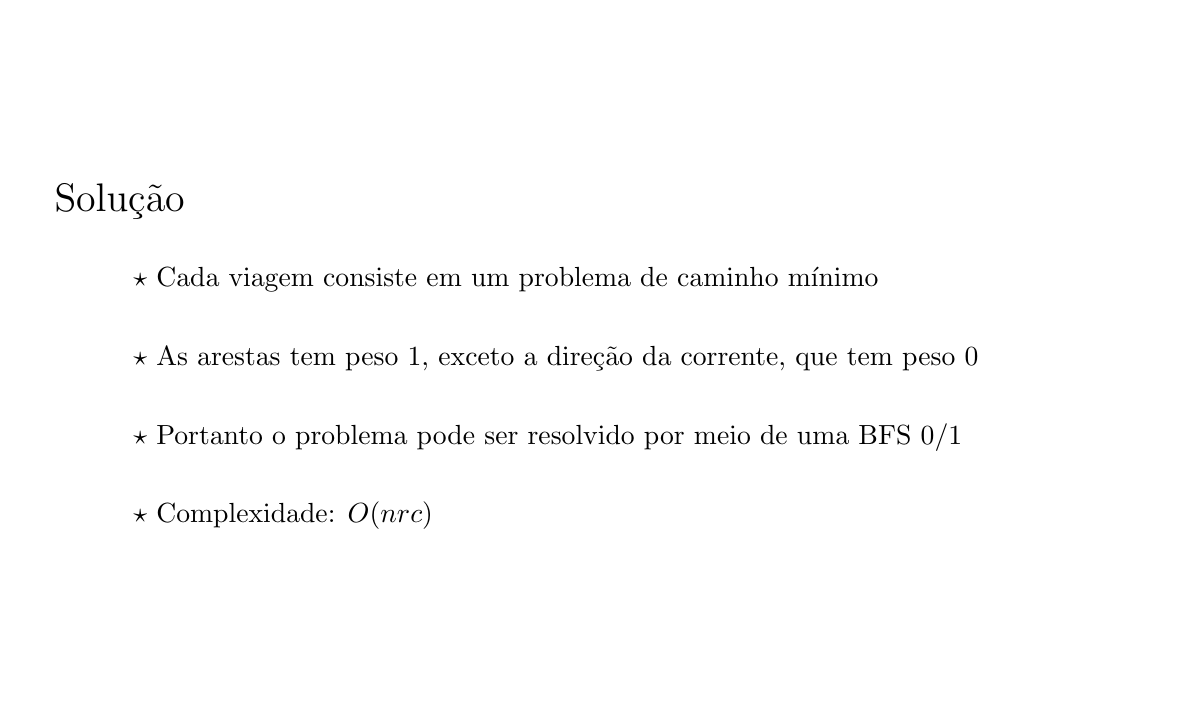
\begin{tikzpicture}
\node[draw,opacity=0] at (0, 0) {x};
\node[draw,opacity=0] at (14, 8) {x};

	\node[anchor=west] (header) at (0, 6.0) { \Large \bbbold{Solução} };


	\node[anchor=west] (a) at (1.0, 5.0) { $\star$ \bbtext{Cada viagem consiste em um problema de caminho mínimo} };


	\node[anchor=west] (b) at (1.0, 4.0) { $\star$ \bbtext{As arestas tem peso $1$, exceto a direção da corrente, que tem peso $0$} };


	\node[anchor=west] (c) at (1.0, 3.0) { $\star$ \bbtext{Portanto o problema pode ser resolvido por meio de uma BFS 0/1} };


	\node[anchor=west] (d) at (1.0, 2.0) { $\star$ \bbbold{Complexidade:} $O(nrc)$ };

\end{tikzpicture}
\end{frame}
\begin{frame}[plain,t]

\inputsnippet{cpp}{10}{29}{codes/437C.cpp}

\end{frame}
\begin{frame}[plain,t]

\inputsnippet{cpp}{31}{50}{codes/437C.cpp}

\end{frame}
\end{document}
